\documentclass{beamer}
\usepackage[utf8]{inputenc}
\usepackage{graphicx,caption,subcaption}
\usepackage{tikz}
\usepackage{pgfplots}
\usepackage{pgf-pie}

\usetikzlibrary{trees}
\usetikzlibrary{mindmap,shadows}

\usetikzlibrary{
	intersections, arrows.meta,
	automata,er,calc,
	backgrounds,
	mindmap,folding,
	patterns,
	decorations.markings,
	fit,
	shapes,matrix,
	positioning,
	shapes.geometric,
	arrows,through
}

\usetheme{CambridgeUS}

\tikzset{
	invisible/.style={opacity=0},
	visible on/.style={alt=#1{}{invisible}},
	alt/.code args={<#1>#2#3}{%
		\alt<#1>{\pgfkeysalso{#2}}{\pgfkeysalso{#3}} % \pgfkeysalso doesn't change the path
	},
} 

\begin{document}
	\title{CRUCEROS}
	\subtitle{Actualización Científica en Matemáticas}
	\author{M.Carmen Plaza Bermejo}
	\institute{UCA}
	\date{Mayo 26, 2020}
	
	%-------------------------------
	
\begin{frame}
\titlepage
\end{frame}
	%-------------------------------
\begin{frame}
\frametitle{Índice}
\tableofcontents
\end{frame}

%-------------------------------

%-------------------------------
\section{Introducción}%%lo que aparece en el índice

\begin{frame}{Tipos de buques}



\begin{center}
	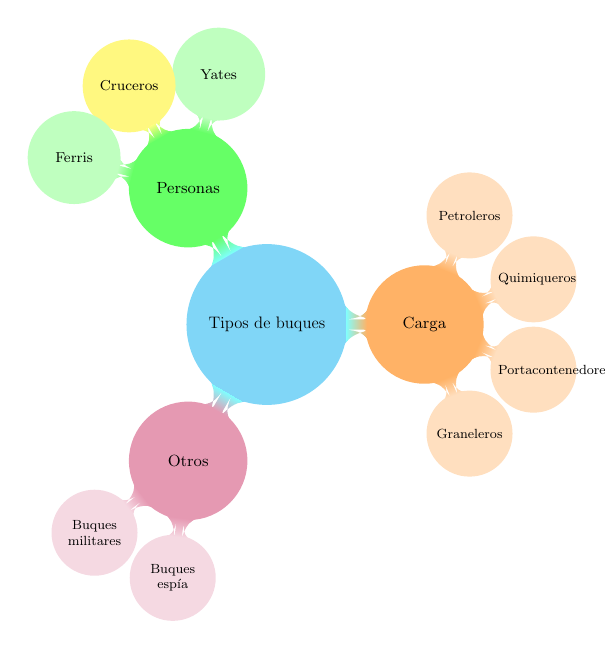
\begin{tikzpicture}[mindmap,scale=0.05,grow cyclic, every node/.style=concept, concept color=cyan!50, align=flush center]
	
	\tikzset{level 1 concept/.append style={ sibling angle=120,level distance = 40cm}}
	\tikzset{level 2 concept/.append style={ sibling angle=45,level distance = 30cm}}
	
	\node [scale=0.5, visible on=<1->] {Tipos de buques}
	child[concept color=purple!40,visible on=<11->]{node[scale=0.65]{Otros}
		child[concept color=purple!15,visible on=<12->]{node [scale=0.6]{Buques militares}}
		child[concept color=purple!15,visible on=<13->]{node[scale=0.6]{Buques espía}}
	}
	child[concept color=orange!60,visible on=<2->] {node[scale=0.65]{Carga}
		child[concept color=orange!25,visible on=<3->]{node[scale=0.6]{Graneleros}}
		child[concept color=orange!25,visible on=<4->]{node[scale=0.6]{Portacontenedores}}
		child[concept color=orange!25,visible on=<5->]{node[scale=0.6]{Quimiqueros}}
		child[concept color=orange!25,visible on=<6->]{node[scale=0.6]{Petroleros}}
	}
	child [concept color=green!60,visible on=<7->]{node[scale=0.65]{Personas}
		child[concept color=green!25,visible on=<8->]{node[scale=0.65]{Yates}}
		child[concept color=yellow!50,visible on=<9->]{node[scale=0.65]{Cruceros}}
		child[concept color=green!25,visible on=<10->]{node[scale=0.65]{Ferris}}
	};
	\end{tikzpicture}
\end{center}
\end{frame}

%-------------------------------

\section{Cruceros}%%lo que aparece en el índice

\begin{frame}{Cruceros}

\begin{center}
	{\scshape \Huge CRUCEROS}
\end{center}

\begin{center}
	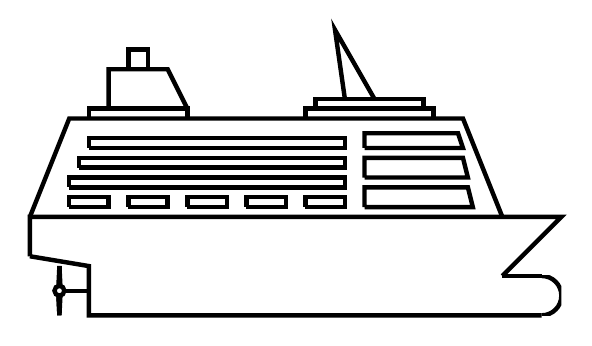
\begin{tikzpicture}[xscale=0.25,yscale=0.25,visible on=<2->]
	
	%casco
	\draw[black, ultra thick](-12,-2)--(-12,0)--(15,0)--(12,-3);
	\draw[black, ultra thick](12,-3)--(14,-3);
	\draw[black, ultra thick](-12,-2)--(-9,-2.5)--(-9,-5)--(14,-5);
	
	%helice
	\draw[black, ultra thick](-9,-3.75)--(-10.25,-3.75);
	\draw[black, ultra thick](-10.5,-3.75)circle(0.25);
	\draw[black, ultra thick](-10.5,-3.5)--(-10.5,-2.5);%pala arriba
	\draw[black, ultra thick](-10.55,-3.5)--(-10.5,-2.5)--(-10.45,-3.5);
	\draw[black, ultra thick](-10.55,-4)--(-10.5,-5);%pala abajo
	\draw[black, ultra thick](-10.55,-4)--(-10.5,-5)--(-10.45,-4);
	
	%bulbo
	\begin{scope}[black, ultra thick]
	\clip (14,-3) rectangle (15,-5);
	\draw (14,-4) circle(1);
	\end{scope}
	
	%estructura
	\draw[black, ultra thick](-12,0)--(-10,5)--(10,5)--(12,0);
	
	%chimeneas
	\draw[black, ultra thick](-9,5)--(-9,5.5)--(-4,5.5)--(-4,5);
	\draw[black, ultra thick](-8,5.5)--(-8,7.5)--(-5,7.5)--(-4,5.5);
	\draw[black, ultra thick](-7,7.5)--(-7,8.5)--(-6,8.5)--(-6,7.5);
	
	\draw[black, ultra thick](2,5)--(2,5.5)--(8.5,5.5)--(8.5,5);
	\draw[black, ultra thick](2.5,5.5)--(2.5,6)--(8,6)--(8,5.5);
	\draw[black, ultra thick](4,6)--(3.5,9.5)--(5.5,6);
	
	%ventanas
	\draw[black, ultra thick](-10,0.5)--(-8,0.5)--(-8,1)--(-10,1)--(-10,0.5);
	\draw[black, ultra thick](-7,0.5)--(-5,0.5)--(-5,1)--(-7,1)--(-7,0.5);
	\draw[black, ultra thick](-4,0.5)--(-2,0.5)--(-2,1)--(-4,1)--(-4,0.5);
	\draw[black, ultra thick](-1,0.5)--(1,0.5)--(1,1)--(-1,1)--(-1,0.5);
	\draw[black, ultra thick](2,0.5)--(4,0.5)--(4,1)--(2,1)--(2,0.5);
	
	\draw[black, ultra thick](-10,1.5)--(4,1.5)--(4,2)--(-10,2)--(-10,1.5);
	\draw[black, ultra thick](-9.5,2.5)--(4,2.5)--(4,3)--(-9.5,3)--(-9.5,2.5);
	\draw[black, ultra thick](-9,3.5)--(4,3.5)--(4,4)--(-9,4)--(-9,3.5);
	
	\draw[black, ultra thick](5,0.5)--(10.5,0.5)--(10.25,1.5)--(5,1.5)--(5,0.5);
	\draw[black, ultra thick](5,2)--(10.25,2)--(10,3)--(5,3)--(5,2);
	\draw[black, ultra thick](5,3.5)--(10,3.5)--(9.75,4.25)--(5,4.25)--(5,3.5);
		
	\end{tikzpicture}
\end{center}
\end{frame}

%-------------------------------
	\section{Compañías}%%lo que aparece en el índice

\begin{frame}{Compañías}


\tikz [font=\footnotesize,
grow=right, level 1/.style={sibling distance=1 cm},
level 2/.style={sibling distance=1cm},
level distance=3.1cm]
\node[color=black,visible on=<1->]{\scshape Compañías}
child[color=black,visible on=<8->]{node{\scshape Royal Caribbean}
	child{node[visible on=<8->]{
\includegraphics[scale=0.2]{RC}}}
}
child [color=black,visible on=<7->]{node{\scshape pullmantur}
	child{node[visible on=<7->]{
\includegraphics[scale=0.15]{PLL}}}
}
child[color=black,visible on=<6->]{node{\scshape MSC Cruceros}
	child{node[visible on=<6->]{
\includegraphics[scale=0.08]{MSC}}}
}
child[color=black,visible on=<5->]{node{\scshape Carnival}
	child{node[visible on=<5->]{
\includegraphics[scale=0.1]{CR}}}
}
child[color=black,visible on=<4->]{node{\scshape Disney}
	child{node[visible on=<4->]{
\includegraphics[scale=0.08]{DY}}}
}
child[color=black,visible on=<3->]{node{\scshape Windstar}
	child{node[visible on=<3->]{
\includegraphics[scale=0.07]{WC}}}
}
child[color=black,visible on=<2->]{node{\scshape Costa Cruceros}
	child{node[visible on=<2->]{
\includegraphics[scale=0.05]{CC}}}
};


\end{frame}

%-------------------------------

\section{Rutas}%%lo que aparece en el índice

\begin{frame}{Rutas principales de los cruceros}

\begin{figure}[h]
	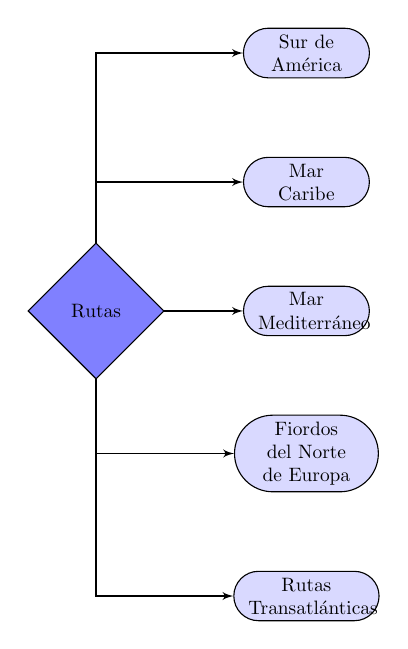
\begin{tikzpicture}
	
	\node[draw,diamond, fill=blue!50, text width=5em, text centered,scale=0.7,visible on=<1->](Rutas){Rutas};
	
	\node[draw,rounded rectangle,right=of Rutas, fill=blue!15, text width=5em, text centered, scale=0.7,visible on=<4->](Med){Mar Mediterráneo};
	\node[draw,rounded rectangle, above=of Med, fill=blue!15, text width=5em, text centered,scale=0.7,visible on=<3->](Caribe){Mar Caribe};
	\node[draw,rounded rectangle, above=of Caribe, fill=blue!15, text width=5em, text centered,scale=0.7,visible on=<2->](Sur){Sur de América};
	\node[draw,rounded rectangle, below=of Med, fill=blue!15, text width=5em, text centered,scale=0.7,visible on=<5->](Fiordos){Fiordos del Norte de Europa};		
	\node[draw,rounded rectangle, below=of Fiordos, fill=blue!15, text width=6em, text centered,scale=0.7,visible on=<6->](Trans){Rutas Transatlánticas};
	
	\tikzstyle{line} = [draw, -latex']
	
	\draw[->, line,visible on=<5->](Rutas)|-(Fiordos);
	\draw[->, line,visible on=<4->](Rutas)--(Med);
	\draw[->, line,visible on=<2->](Rutas)|-(Sur);
	\draw[->, line,visible on=<3->](Rutas)|-(Caribe);
	\draw[->, line,visible on=<6->](Rutas)|-(Trans);
	
	
	\end{tikzpicture}
\end{figure}

\end{frame}


\begin{frame}{Rutas principales de los cruceros}

\begin{figure}[h!]
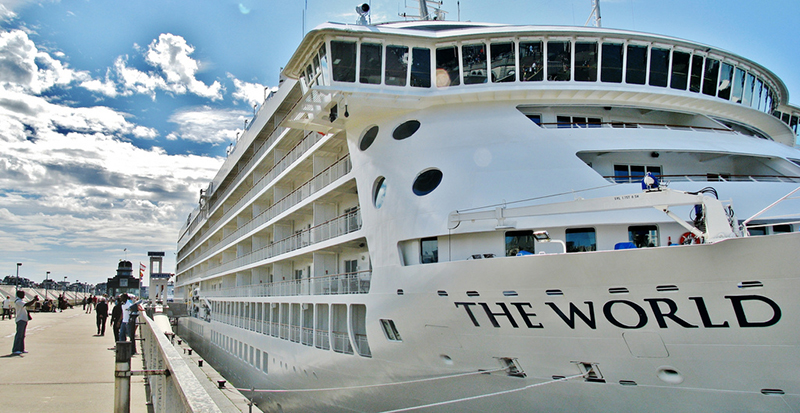
\includegraphics{world}
\caption{The world}
\end{figure}
\end{frame}

\begin{frame}{Rutas principales de los cruceros}

\begin{figure}
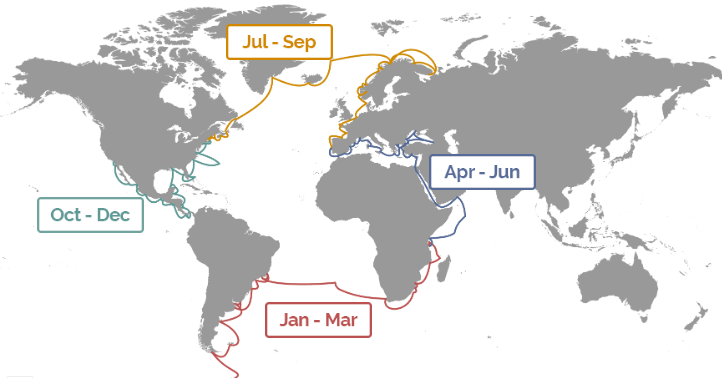
\includegraphics[scale=0.6]{itin}
\caption{Itinerario The world, 2021}
\end{figure}
\end{frame}

%-------------------------------

\section{Procedencia pasajeros}%%lo que aparece en el índice

\begin{frame}{Procedencia de los pasajeros de cruceros}

\begin{center}
	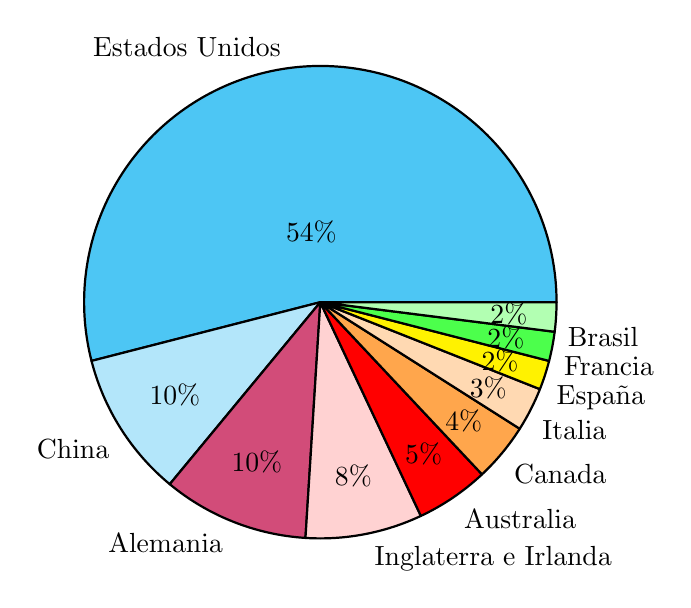
\begin{tikzpicture}
	\pie[color={cyan!70,cyan!30, purple!70,pink!70,red,orange!70,orange!30,yellow,green!70,green!30}]
	{54/Estados Unidos,10/China,10/Alemania,8/Inglaterra e Irlanda,5/Australia,4/Canada,3/Italia,2/España,2/Francia,2/Brasil}
	
	\end{tikzpicture}
	
\end{center}

\end{frame}
%-------------------------------
\section{Evolución }%%lo que aparece en el índice

\begin{frame}{Evolución }

\begin{figure}
	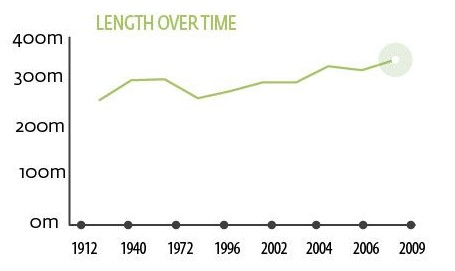
\includegraphics[scale=0.5]{lenght}
\end{figure}

\end{frame}	

\begin{frame}{Evolución }

\begin{figure}

\centering
\begin{subfigure}[h]{0.35\textwidth} 
	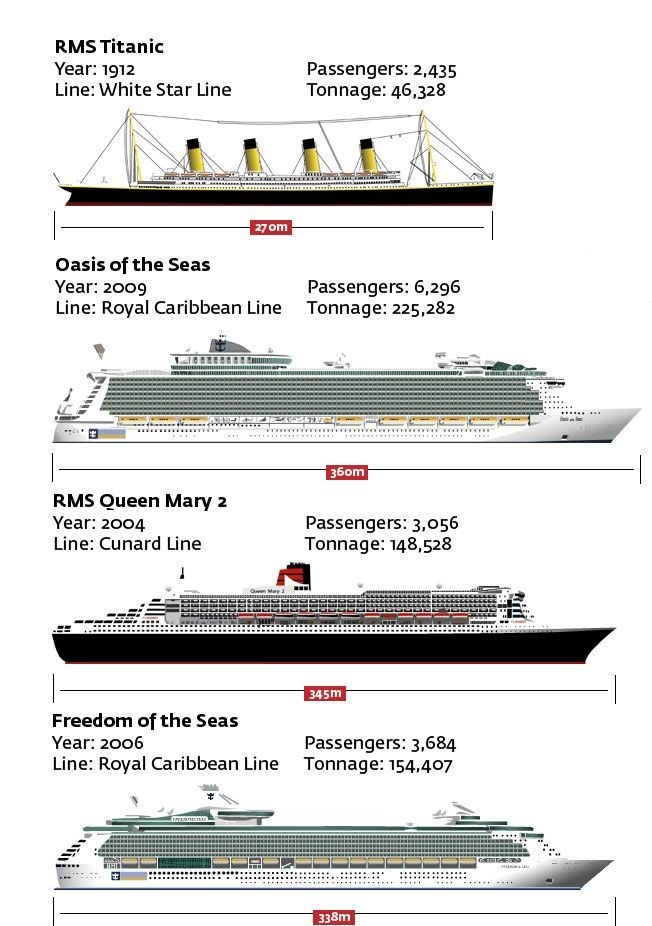
\includegraphics[width=\textwidth]{b1}
	
\end{subfigure}       
\begin{subfigure}[h]{0.35\textwidth} 
	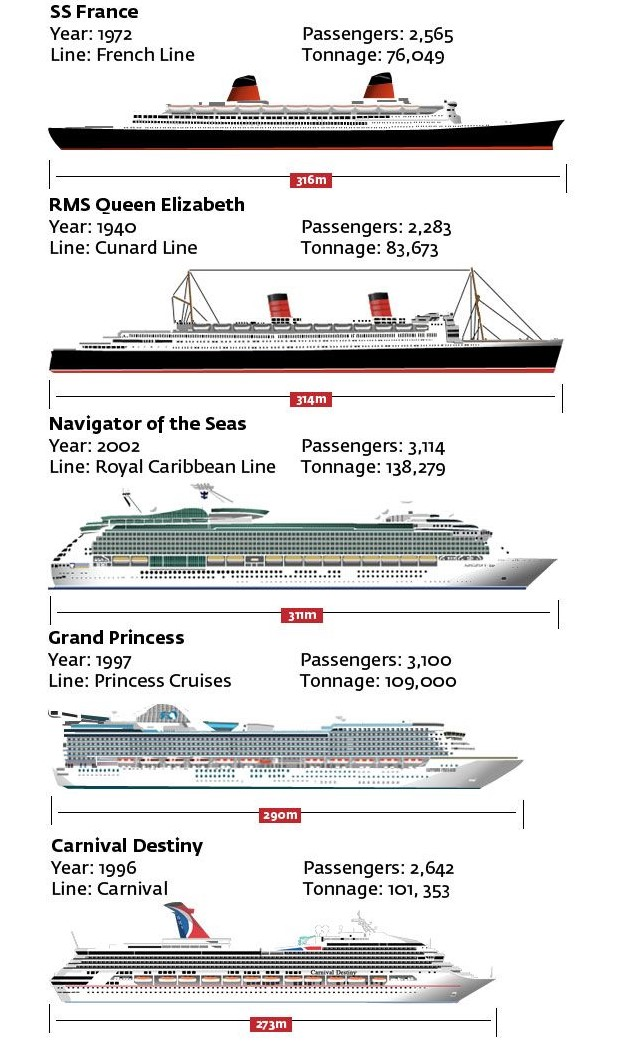
\includegraphics[width=\textwidth]{b2}
	
\end{subfigure}

\end{figure}

\end{frame}	

\begin{frame}{Evolución}

\begin{figure}
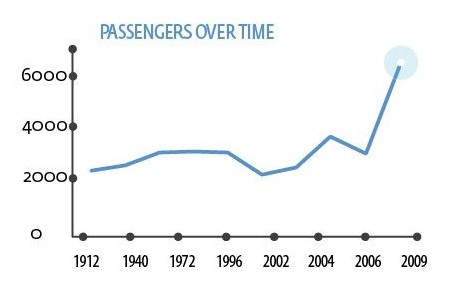
\includegraphics[scale=0.5]{pass}
\end{figure}

\end{frame}
%-------------------------------
\section{Cruceros más grandes del mundo}

\begin{frame}{Cruceros más grandes del mundo}

\begin{figure}[h]
	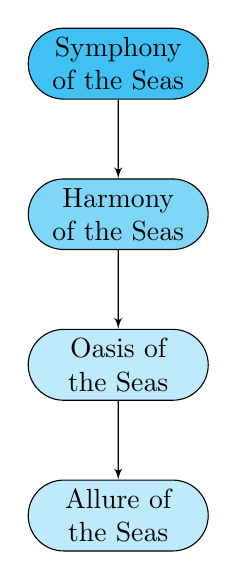
\begin{tikzpicture}
	
	\node[draw,rounded rectangle, fill=cyan!75, text width=5em, text centered,scale=1,visible on=<2->](S){Symphony of the Seas};
	\node[draw,rounded rectangle,below=of S, fill=cyan!50, text width=5em, text centered, scale=1,visible on=<3->](H){Harmony of the Seas};
	\node[draw,rounded rectangle, below=of H, fill=cyan!25, text width=5em, text centered,scale=1,visible on=<4->](O){Oasis of the Seas};
	\node[draw,rounded rectangle, below=of O, fill=cyan!25, text width=5em, text centered,scale=1,visible on=<4->](A){Allure of the Seas};
	
	\tikzstyle{line} = [draw, -latex']
	
	\draw[->, line,visible on=<3->](S)--(H);
	\draw[->, line,visible on=<4->](H)--(O);
	\draw[->, line,visible on=<4->](O)--(A);
	
	
	\end{tikzpicture}
\end{figure}


\end{frame}
\begin{frame}{Cruceros más grandes del mundo}

\begin{center}
	\begin{figure}
		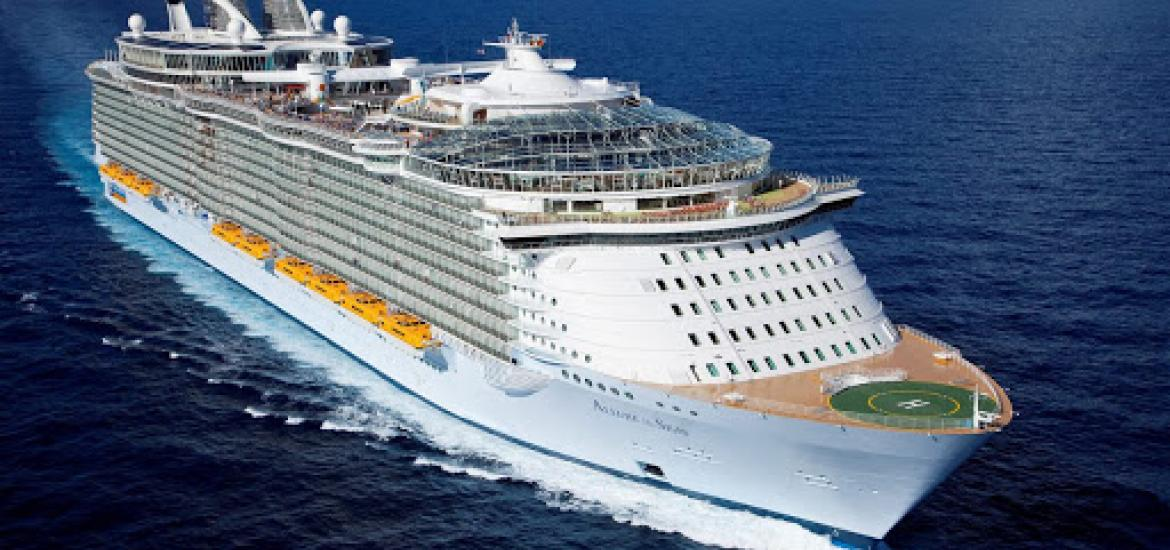
\includegraphics[scale=0.35]{allure}
	\end{figure}
\end{center}
\end{frame}

\begin{frame}{Cruceros más grandes del mundo}

\begin{center}
\begin{figure}
	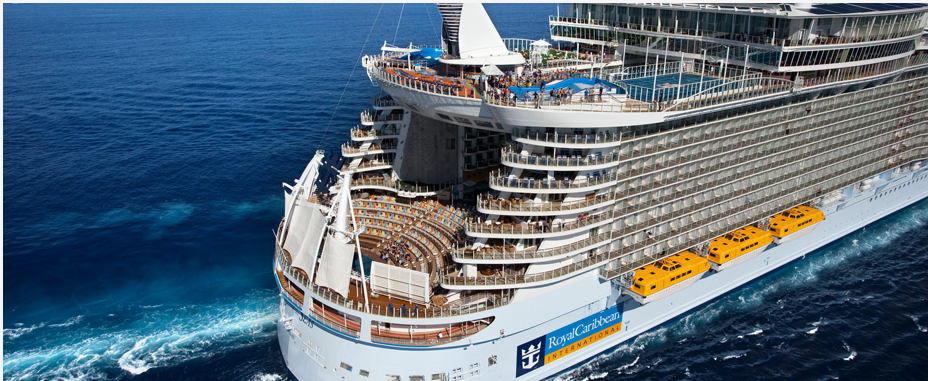
\includegraphics[scale=0.5]{allure1}
\end{figure}
\end{center}
\end{frame}
%-------------------------------
\section{Reparaciones}%%lo que aparece en el índice


\begin{frame}{Reparaciones}
\begin{center}
	{\scshape \Huge CARNIVAL SUNRISE}
\end{center}

\begin{figure}
	\centering
	\begin{subfigure}[h]{0.45\textwidth}
		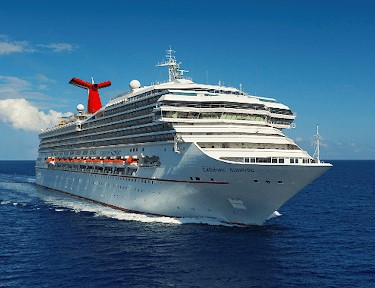
\includegraphics[width=\textwidth]{sr2}
		
	\end{subfigure}       
	\begin{subfigure}[h]{0.45\textwidth} 
		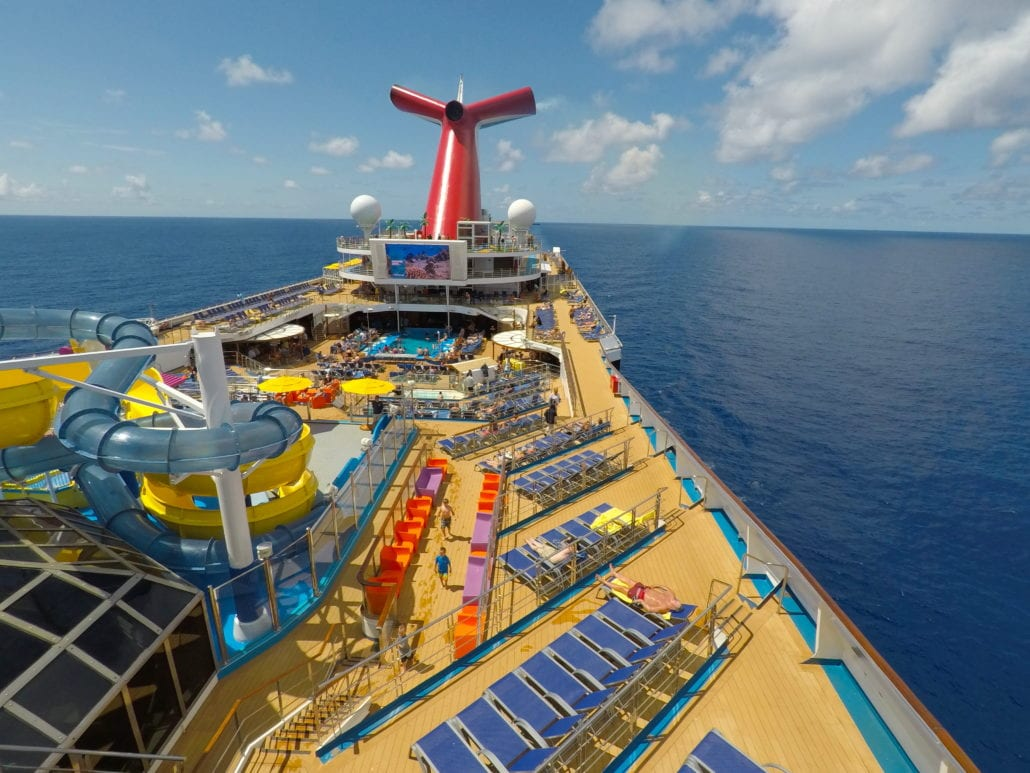
\includegraphics[width=\textwidth]{sr1}
	\end{subfigure}
	\end{figure}
\end{frame}

\begin{frame}{Reparaciones}
\begin{center}
	{\scshape \Huge CARNIVAL SUNRISE}
\end{center}

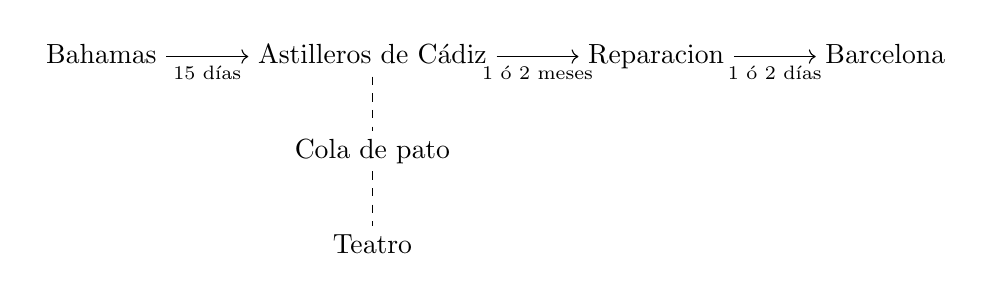
\begin{tikzpicture}
\matrix (m) [matrix of math nodes,ampersand replacement=\&, row sep=2em, %reemplazar ampersand
column sep=1.5em, text height=1.5ex, text depth=0.25ex]
{ \mbox{Bahamas}\& \& \mbox{Astilleros de Cádiz} \& \& \mbox{Reparacion} \& \& \mbox{Barcelona}\\
	\&  \& \mbox{Cola de pato}  \& \&    \\ 
	\&  \& \mbox{Teatro}  \& \&    \\ };

\path[->, font=\scriptsize](m-1-1) edge node[below]{15 días} (m-1-3)
(m-1-3) edge node[below]{1 ó 2 meses} (m-1-5)
(m-1-5) edge node[below]{1 ó 2 días} (m-1-7);
\path[dashed] (m-1-3) edge (m-2-3);
\path[dashed] (m-2-3) edge (m-3-3);
\end{tikzpicture}

\end{frame}	


\begin{frame}{Reparaciones}

\begin{figure}
\centering
\begin{subfigure}[h]{0.45\textwidth} 
	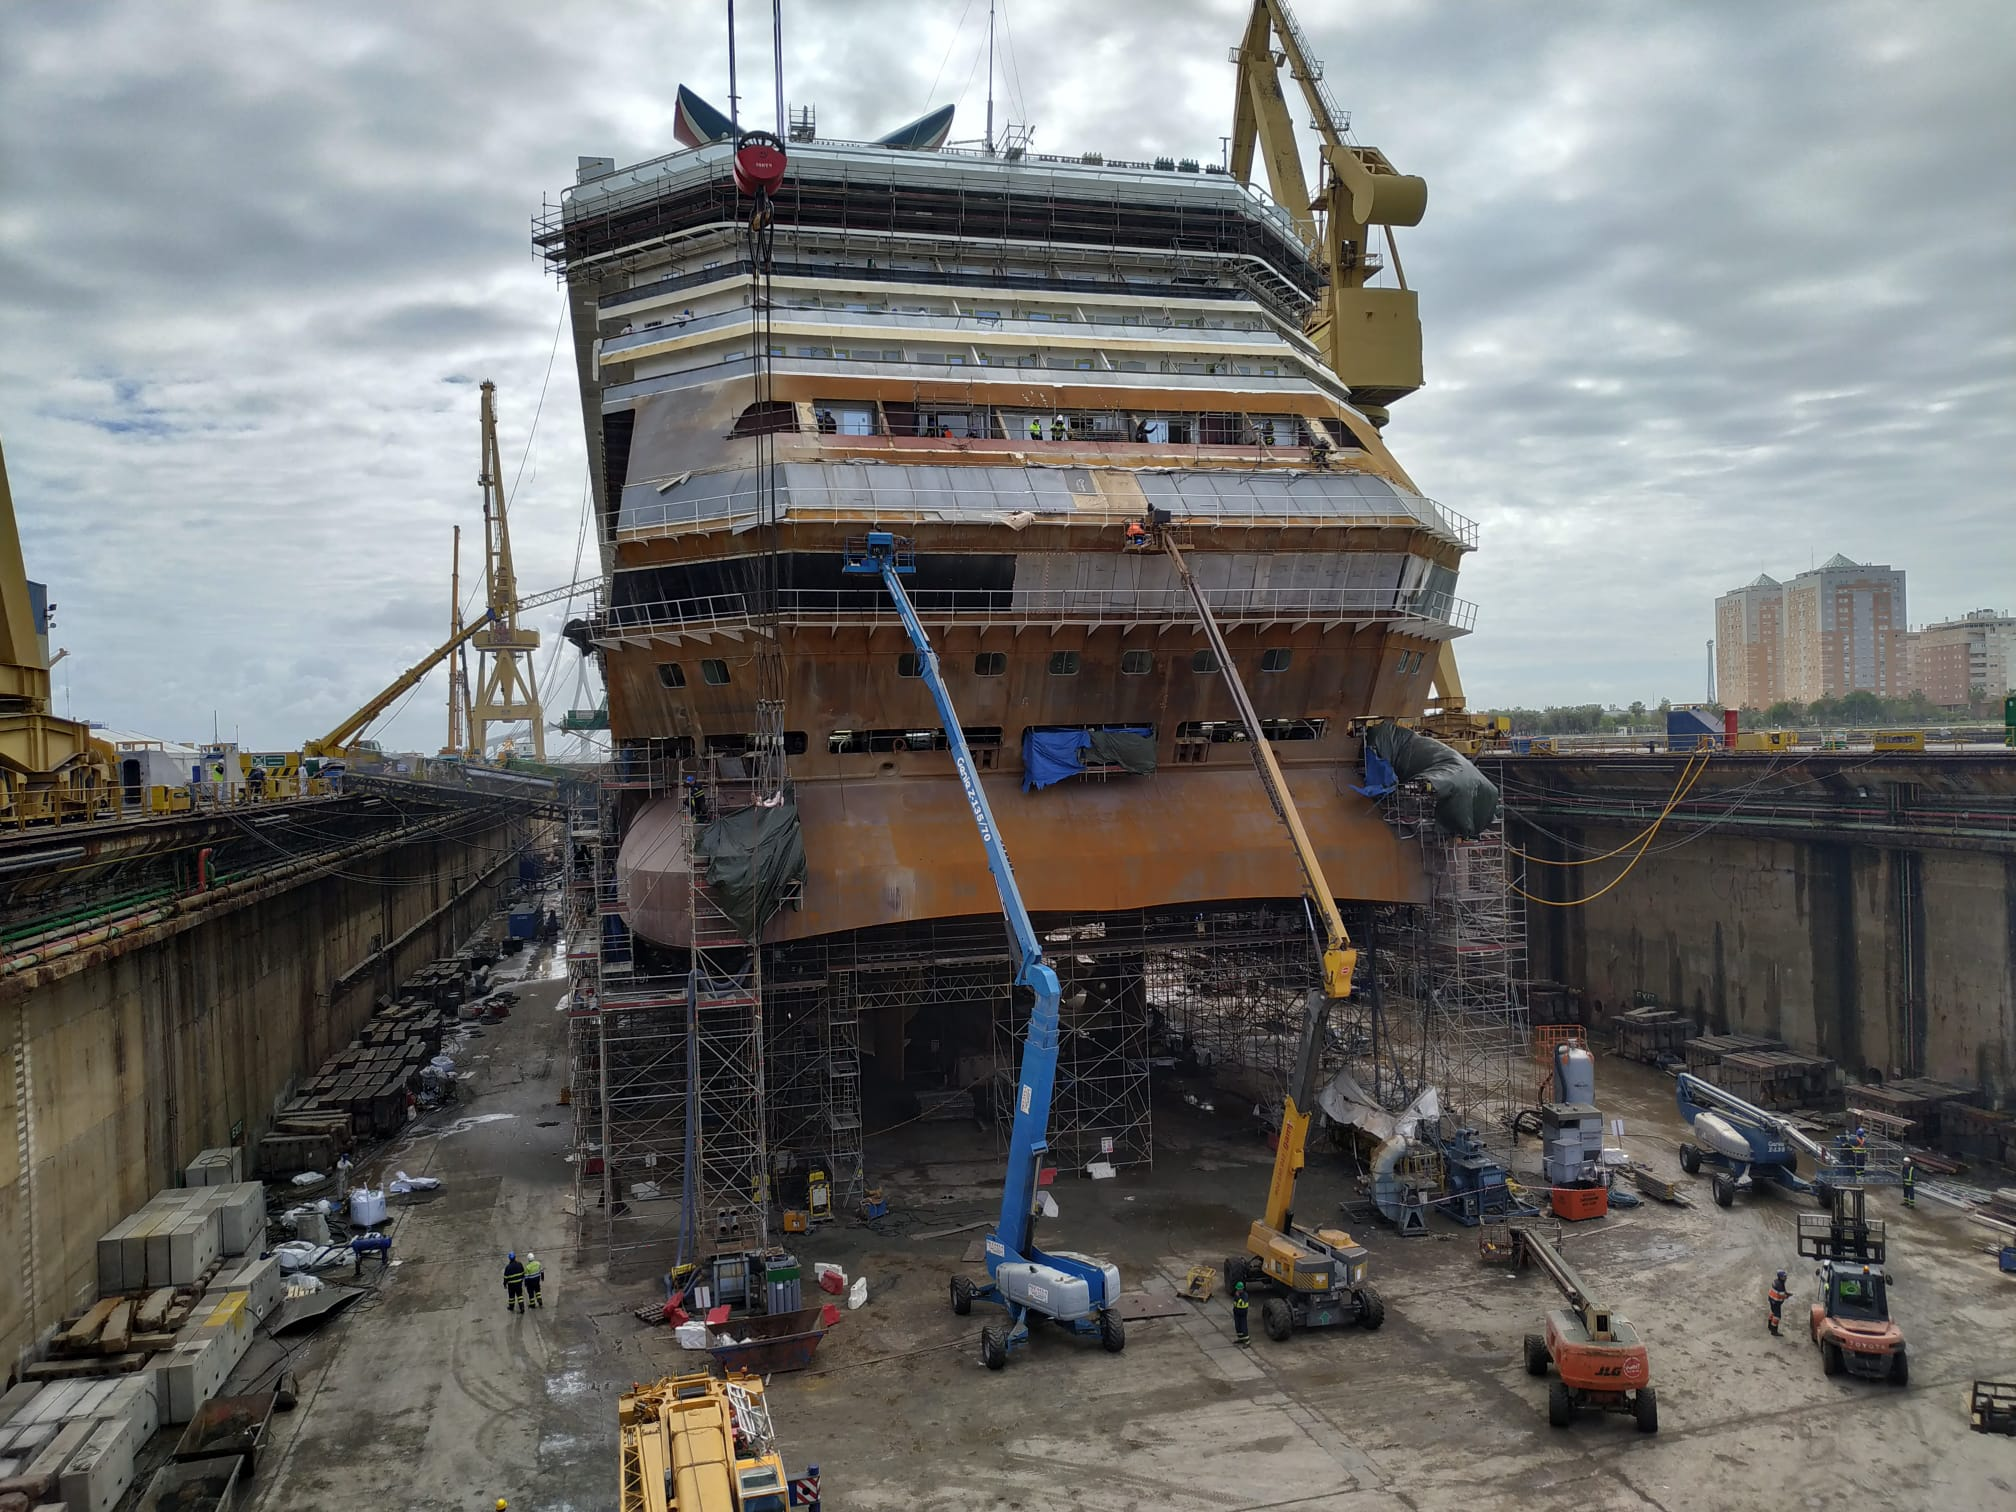
\includegraphics[width=\textwidth]{pato1}
	
\end{subfigure}       
\begin{subfigure}[h]{0.45\textwidth} 
	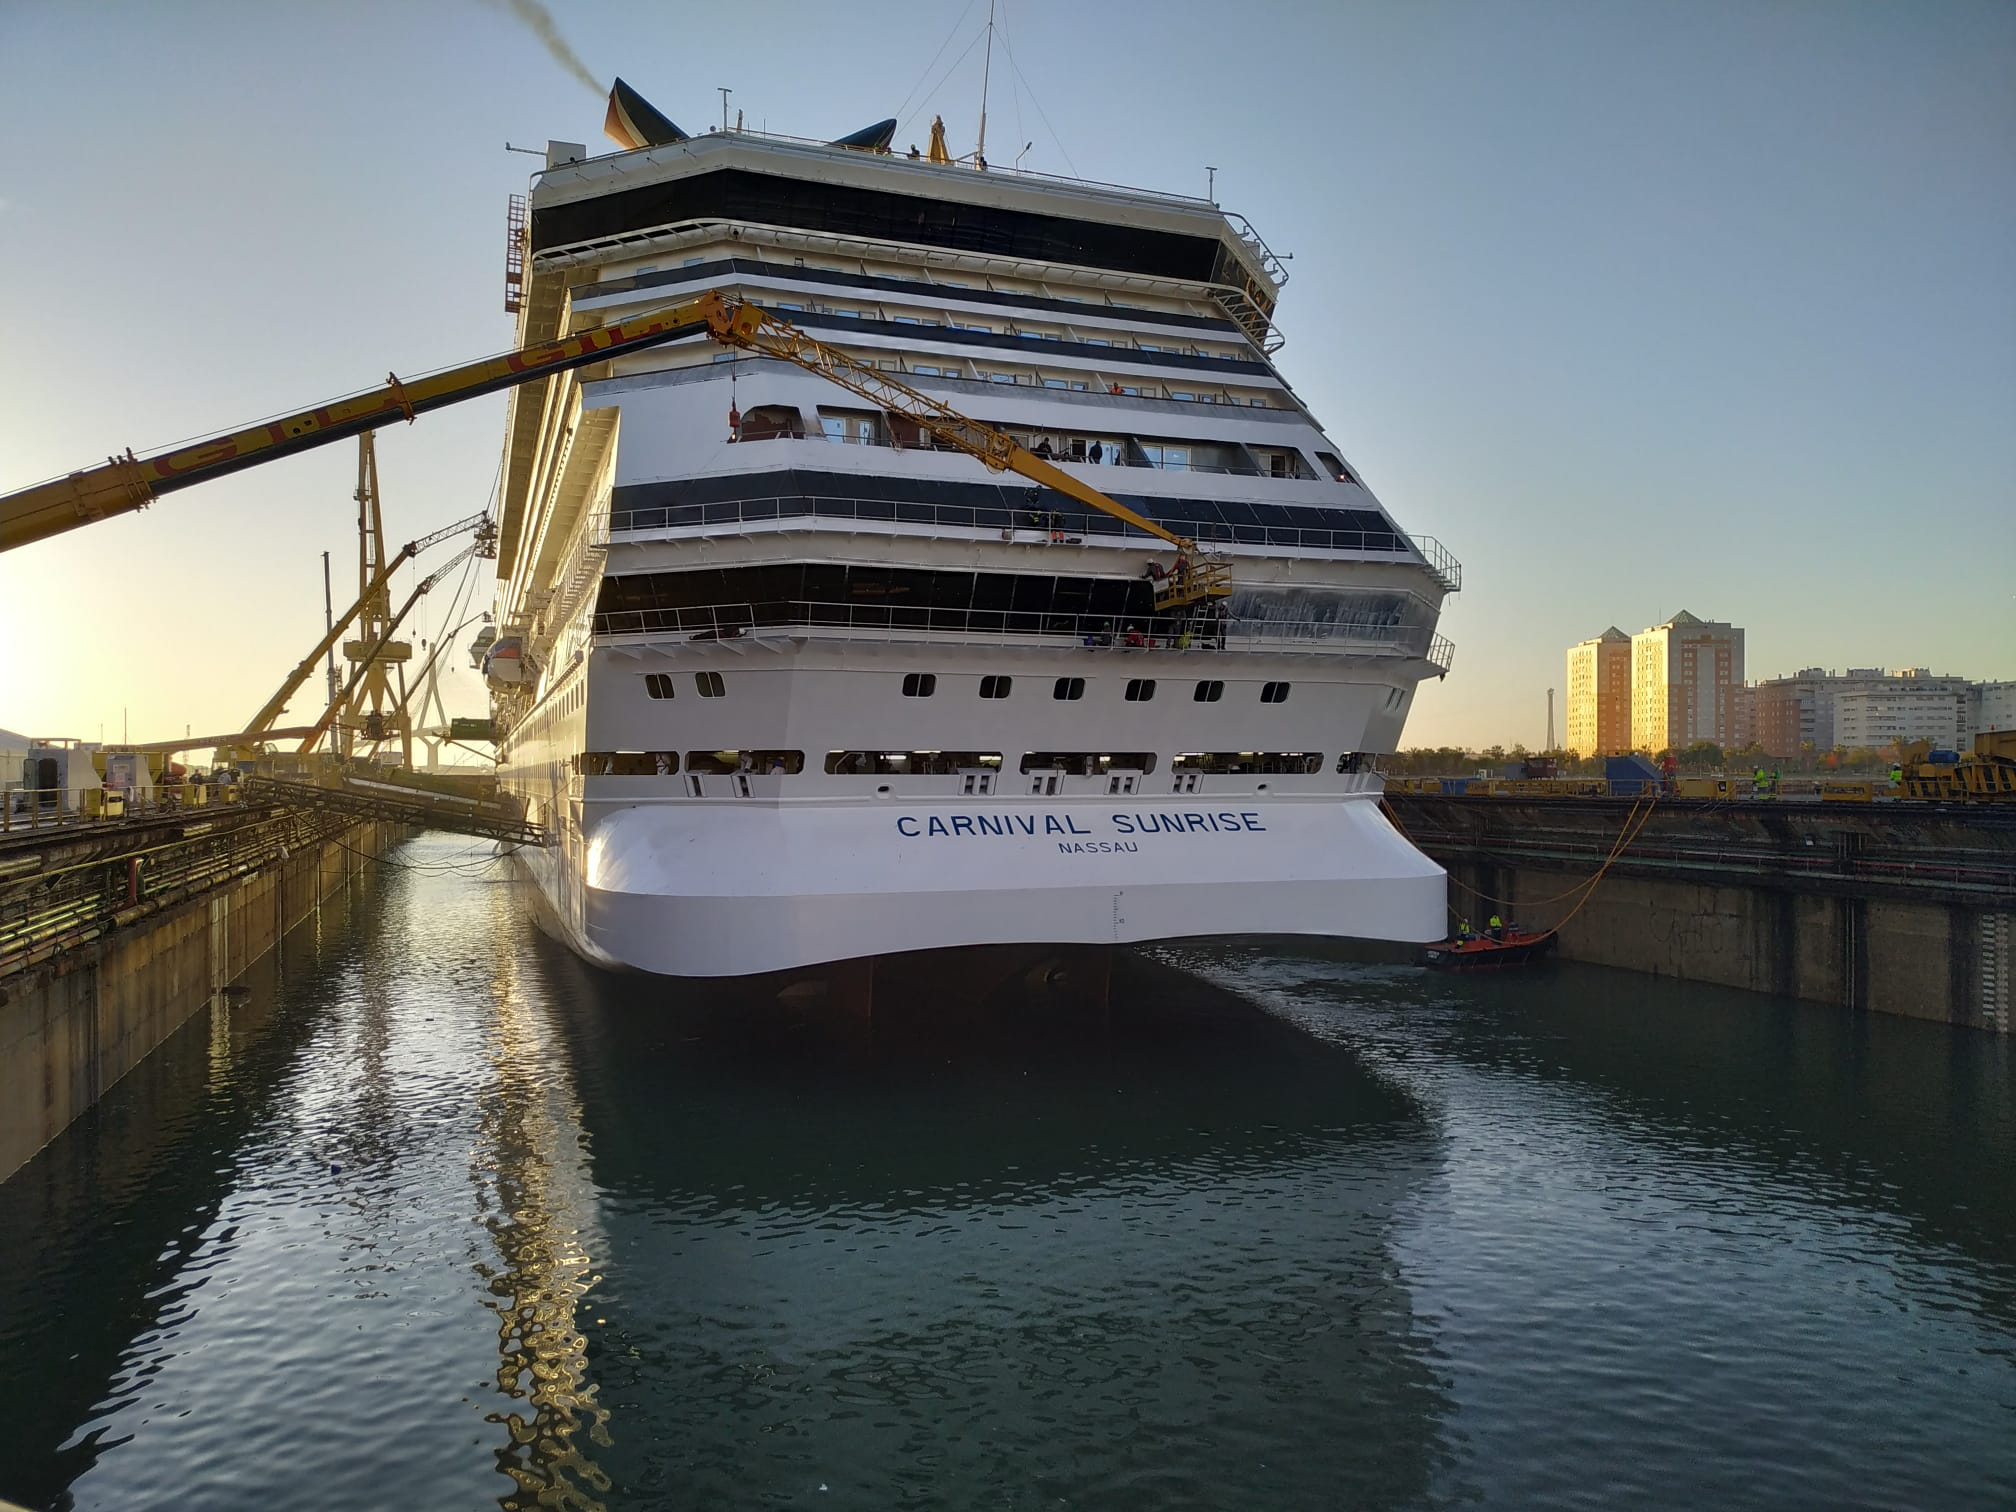
\includegraphics[width=\textwidth]{pato2}
	
\end{subfigure}

\caption{Construcción cola de pato}
\end{figure}

\end{frame}

\begin{frame}{Reparaciones}

\begin{figure}
\centering
\begin{subfigure}[h]{0.5\textwidth} 
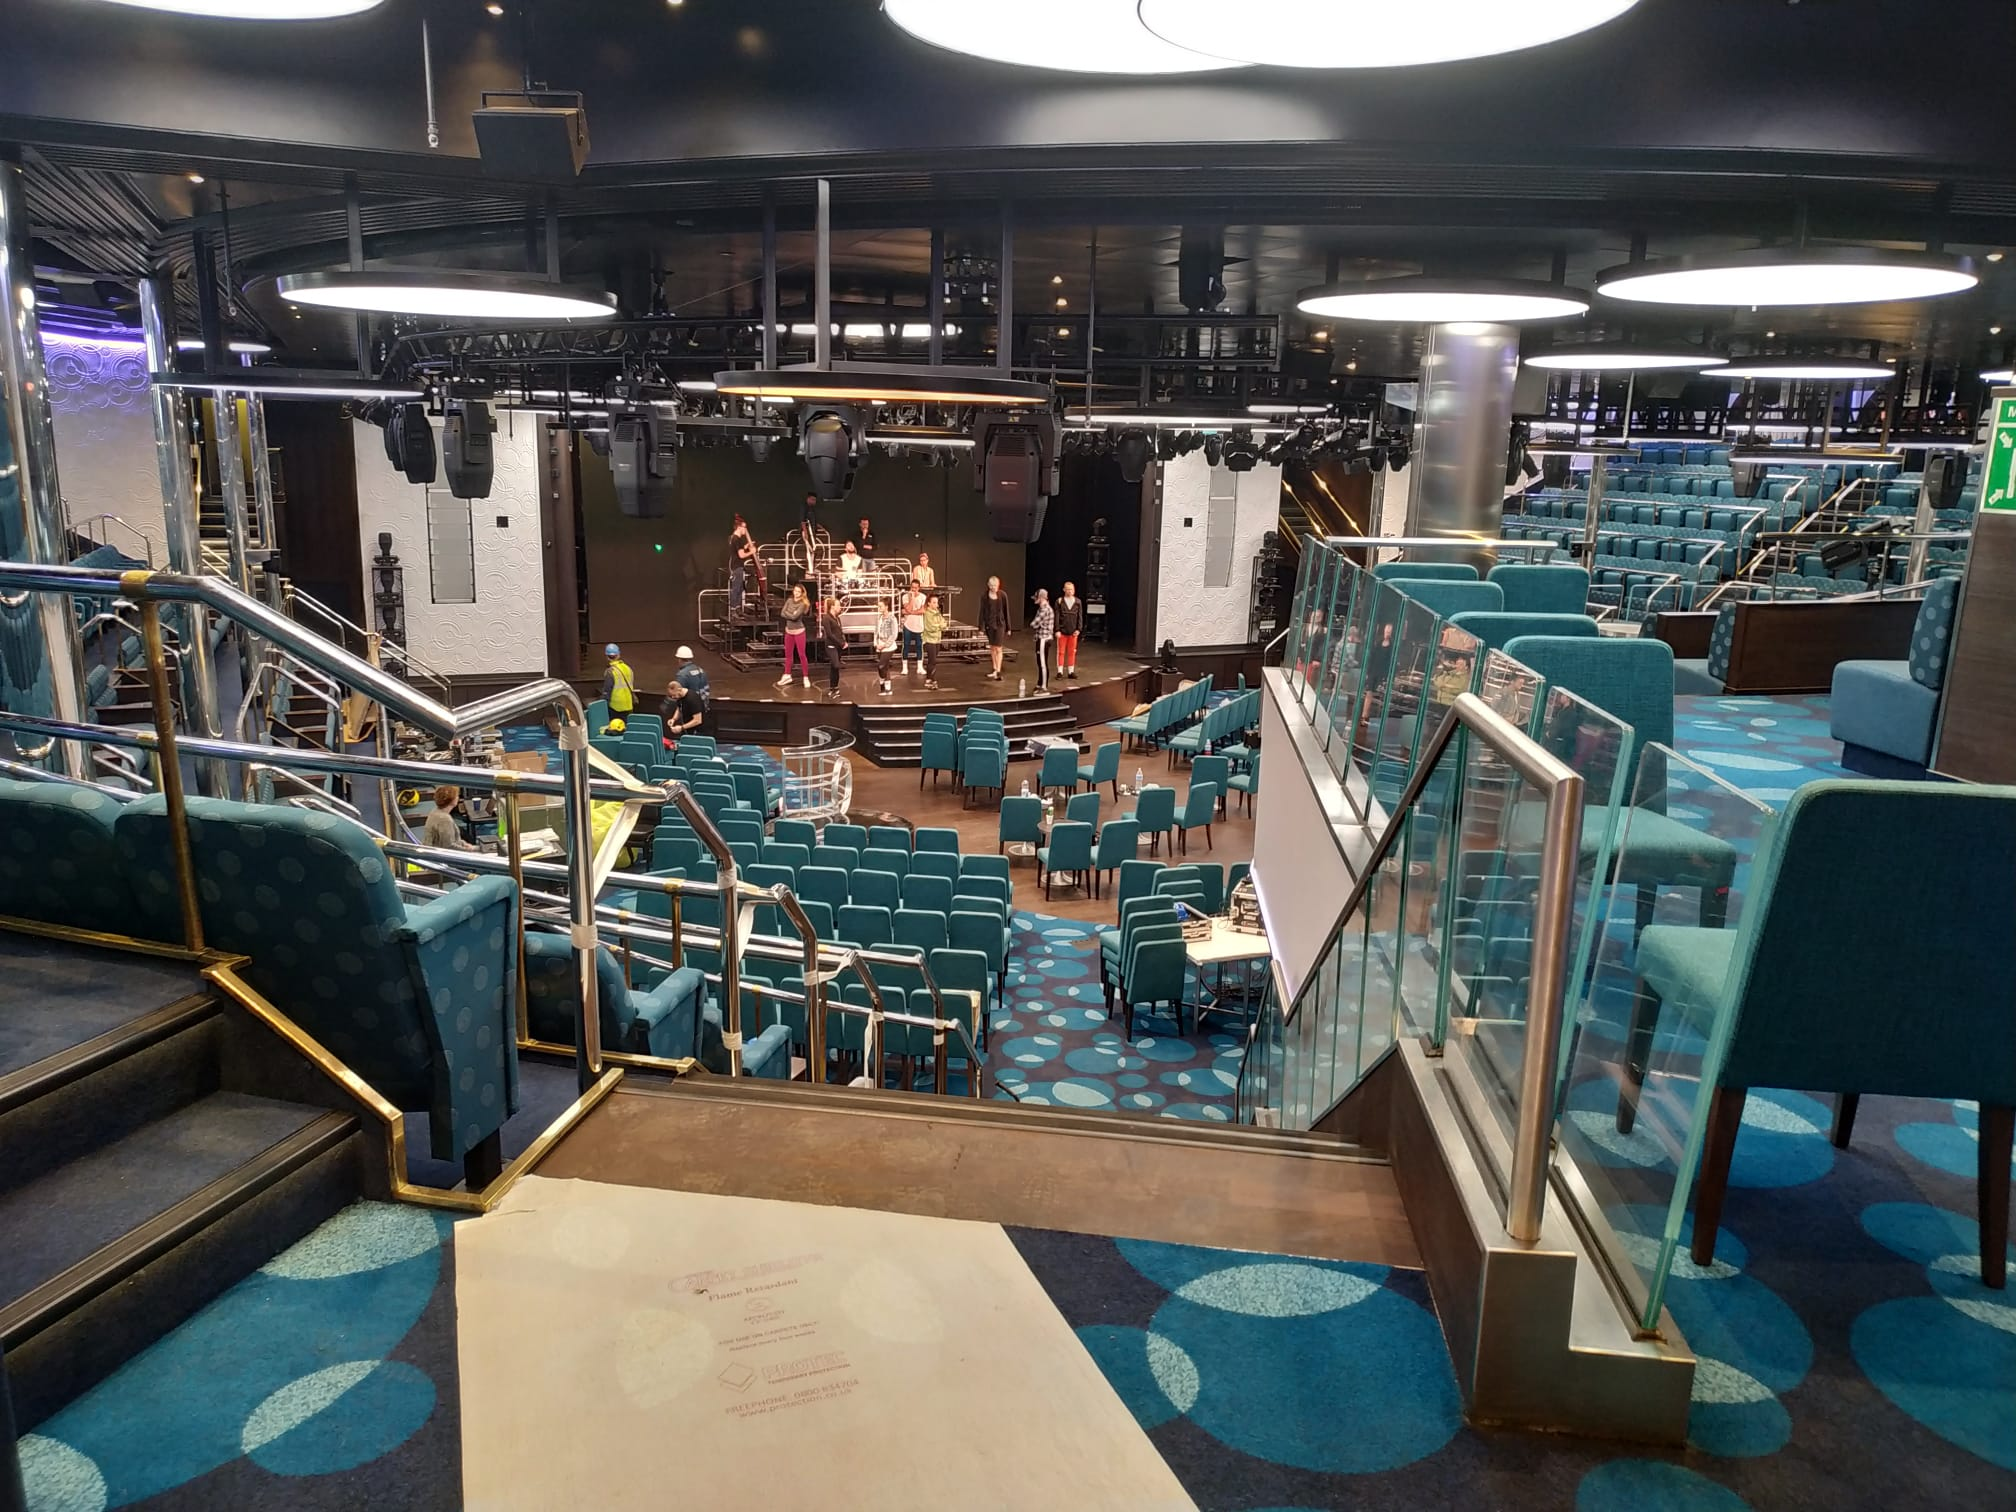
\includegraphics[width=\textwidth]{teatro}
\label{Teatro reparado}
\caption{Teatro reformado}
\end{subfigure}       
\begin{subfigure}[h]{0.45\textwidth} 
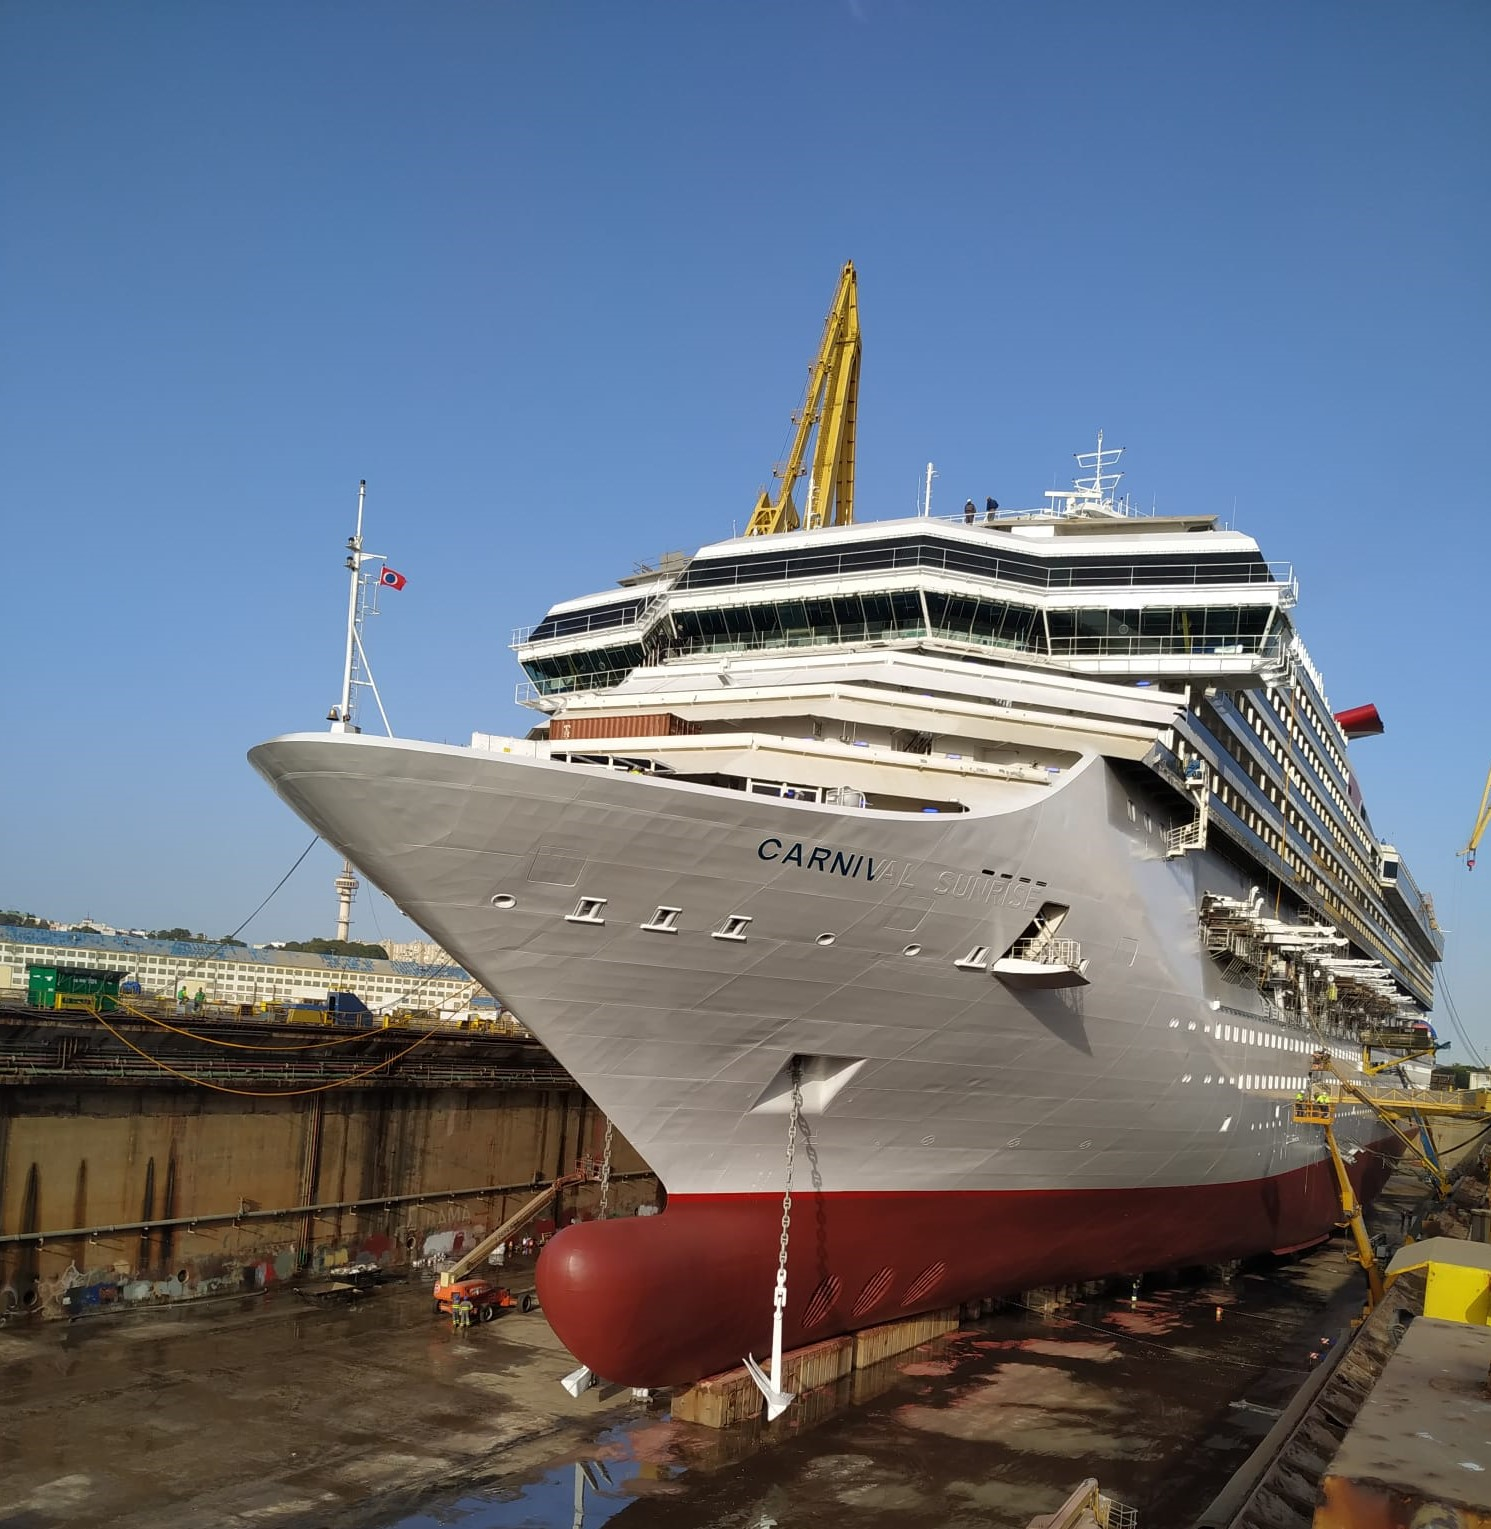
\includegraphics[width=\textwidth]{carn}
\label{Pintura}
\caption{Pintura casco}
\end{subfigure}
\end{figure}

\end{frame}	

\begin{frame}{Reparaciones}
\begin{center}
{\scshape \Huge OASIS OF THE SEAS}
\end{center}
\begin{figure}
	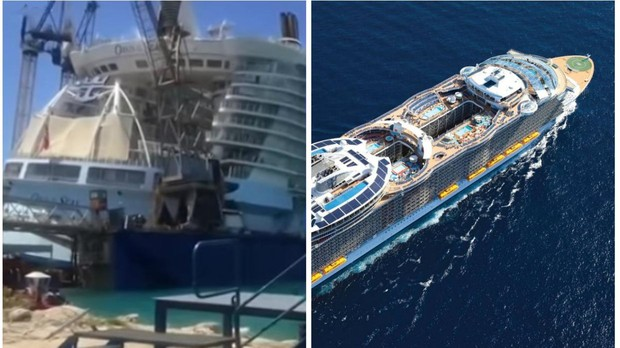
\includegraphics[scale=0.5]{oa1}
	\caption{Oasis of the seas}
\end{figure}

\end{frame}

	

%-------------------------------
\begin{frame}
\begin{center}
	{\scshape \Huge ¡GRACIAS POR \\ SU ATENCIÓN!}
\end{center}
\end{frame}
%-------------------------------
\begin{frame}
\titlepage
\end{frame}
%-------------------------------	
	
\end{document}